\documentclass[12pt,letterpaper]{article}
\usepackage{graphicx,textcomp}
\usepackage{natbib}
\usepackage{setspace}
\usepackage{fullpage}
\usepackage{color}
\usepackage[reqno]{amsmath}
\usepackage{amsthm}
\usepackage{fancyvrb}
\usepackage{amssymb,enumerate}
\usepackage[all]{xy}
\usepackage{endnotes}
\usepackage{lscape}
\newtheorem{com}{Comment}
\usepackage{float}
\usepackage{hyperref}
\newtheorem{lem} {Lemma}
\newtheorem{prop}{Proposition}
\newtheorem{thm}{Theorem}
\newtheorem{defn}{Definition}
\newtheorem{cor}{Corollary}
\newtheorem{obs}{Observation}
\usepackage[compact]{titlesec}
\usepackage{dcolumn}
\usepackage{tikz}
\usetikzlibrary{arrows}
\usepackage{multirow}
\usepackage{xcolor}
\newcolumntype{.}{D{.}{.}{-1}}
\newcolumntype{d}[1]{D{.}{.}{#1}}
\definecolor{light-gray}{gray}{0.65}
\usepackage{url}
\usepackage{listings}
\usepackage{color}

\definecolor{codegreen}{rgb}{0,0.6,0}
\definecolor{codegray}{rgb}{0.5,0.5,0.5}
\definecolor{codepurple}{rgb}{0.58,0,0.82}
\definecolor{backcolour}{rgb}{0.95,0.95,0.92}

\lstdefinestyle{mystyle}{
	backgroundcolor=\color{backcolour},   
	commentstyle=\color{codegreen},
	keywordstyle=\color{magenta},
	numberstyle=\tiny\color{codegray},
	stringstyle=\color{codepurple},
	basicstyle=\footnotesize,
	breakatwhitespace=false,         
	breaklines=true,                 
	captionpos=b,                    
	keepspaces=true,                 
	numbers=left,                    
	numbersep=5pt,                  
	showspaces=false,                
	showstringspaces=false,
	showtabs=false,                  
	tabsize=2
}
\lstset{style=mystyle}
\newcommand{\Sref}[1]{Section~\ref{#1}}
\newtheorem{hyp}{Hypothesis}

\title{\textbf{MS Contribution to:} Lee, C. (2019). China’s Energy Diplomacy: Does Chinese Foreign Policy Favor Oil-Producing Countries? Foreign Policy Analysis, 15(4), 570–588. https://doi.org/10.1093/fpa/orz011

}
\date{Due: March 31, 2024}
\author{Applied Stats II \\ \vspace{\baselineskip}
	\textbf{Maiia Skrypnyk 23371609}}

\begin{document}
	\maketitle

\section{Twist 1: Plots}

\textbf{Loading the data:}
\lstinputlisting[language=R, firstline=14, lastline=17]{Twist_Lee_MS.R} 


\noindent \textbf{Figure 2 Twist:}

\lstinputlisting[language=R, firstline=20, lastline=92]{Twist_Lee_MS.R}  


\begin{figure}[H]
    \centering
    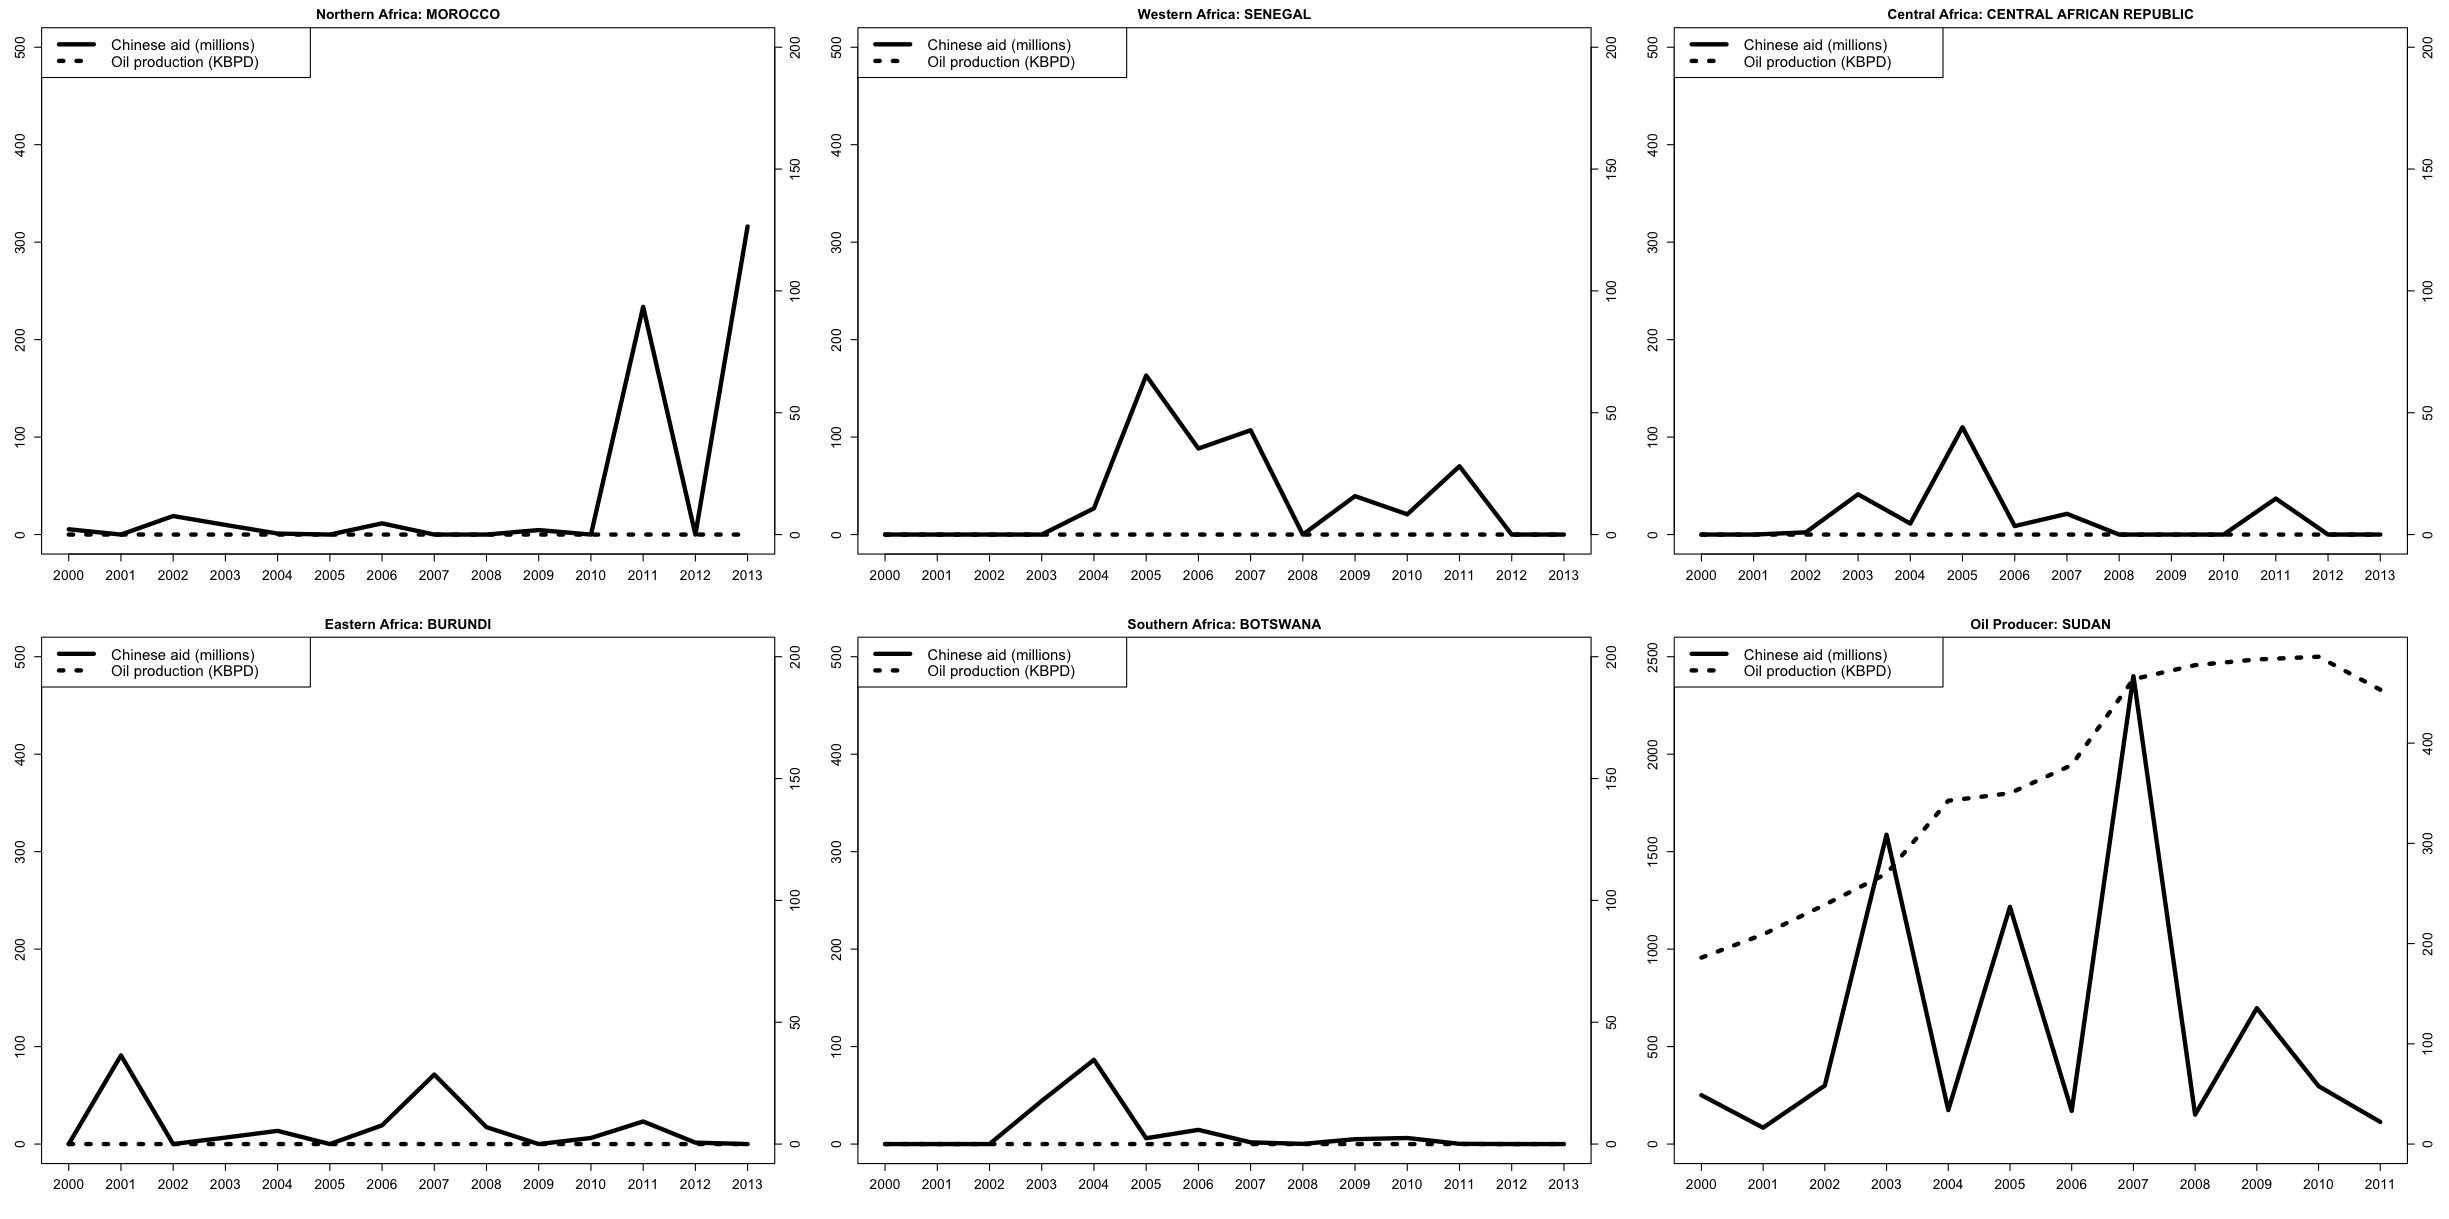
\includegraphics[width=1\linewidth]{figure2MS.png}
\end{figure}

\newpage
\textbf{Model 1 Twist:}

\lstinputlisting[language=R, firstline=97, lastline=131]{Twist_Lee_MS.R}  

\begin{figure}[H]
    \centering
    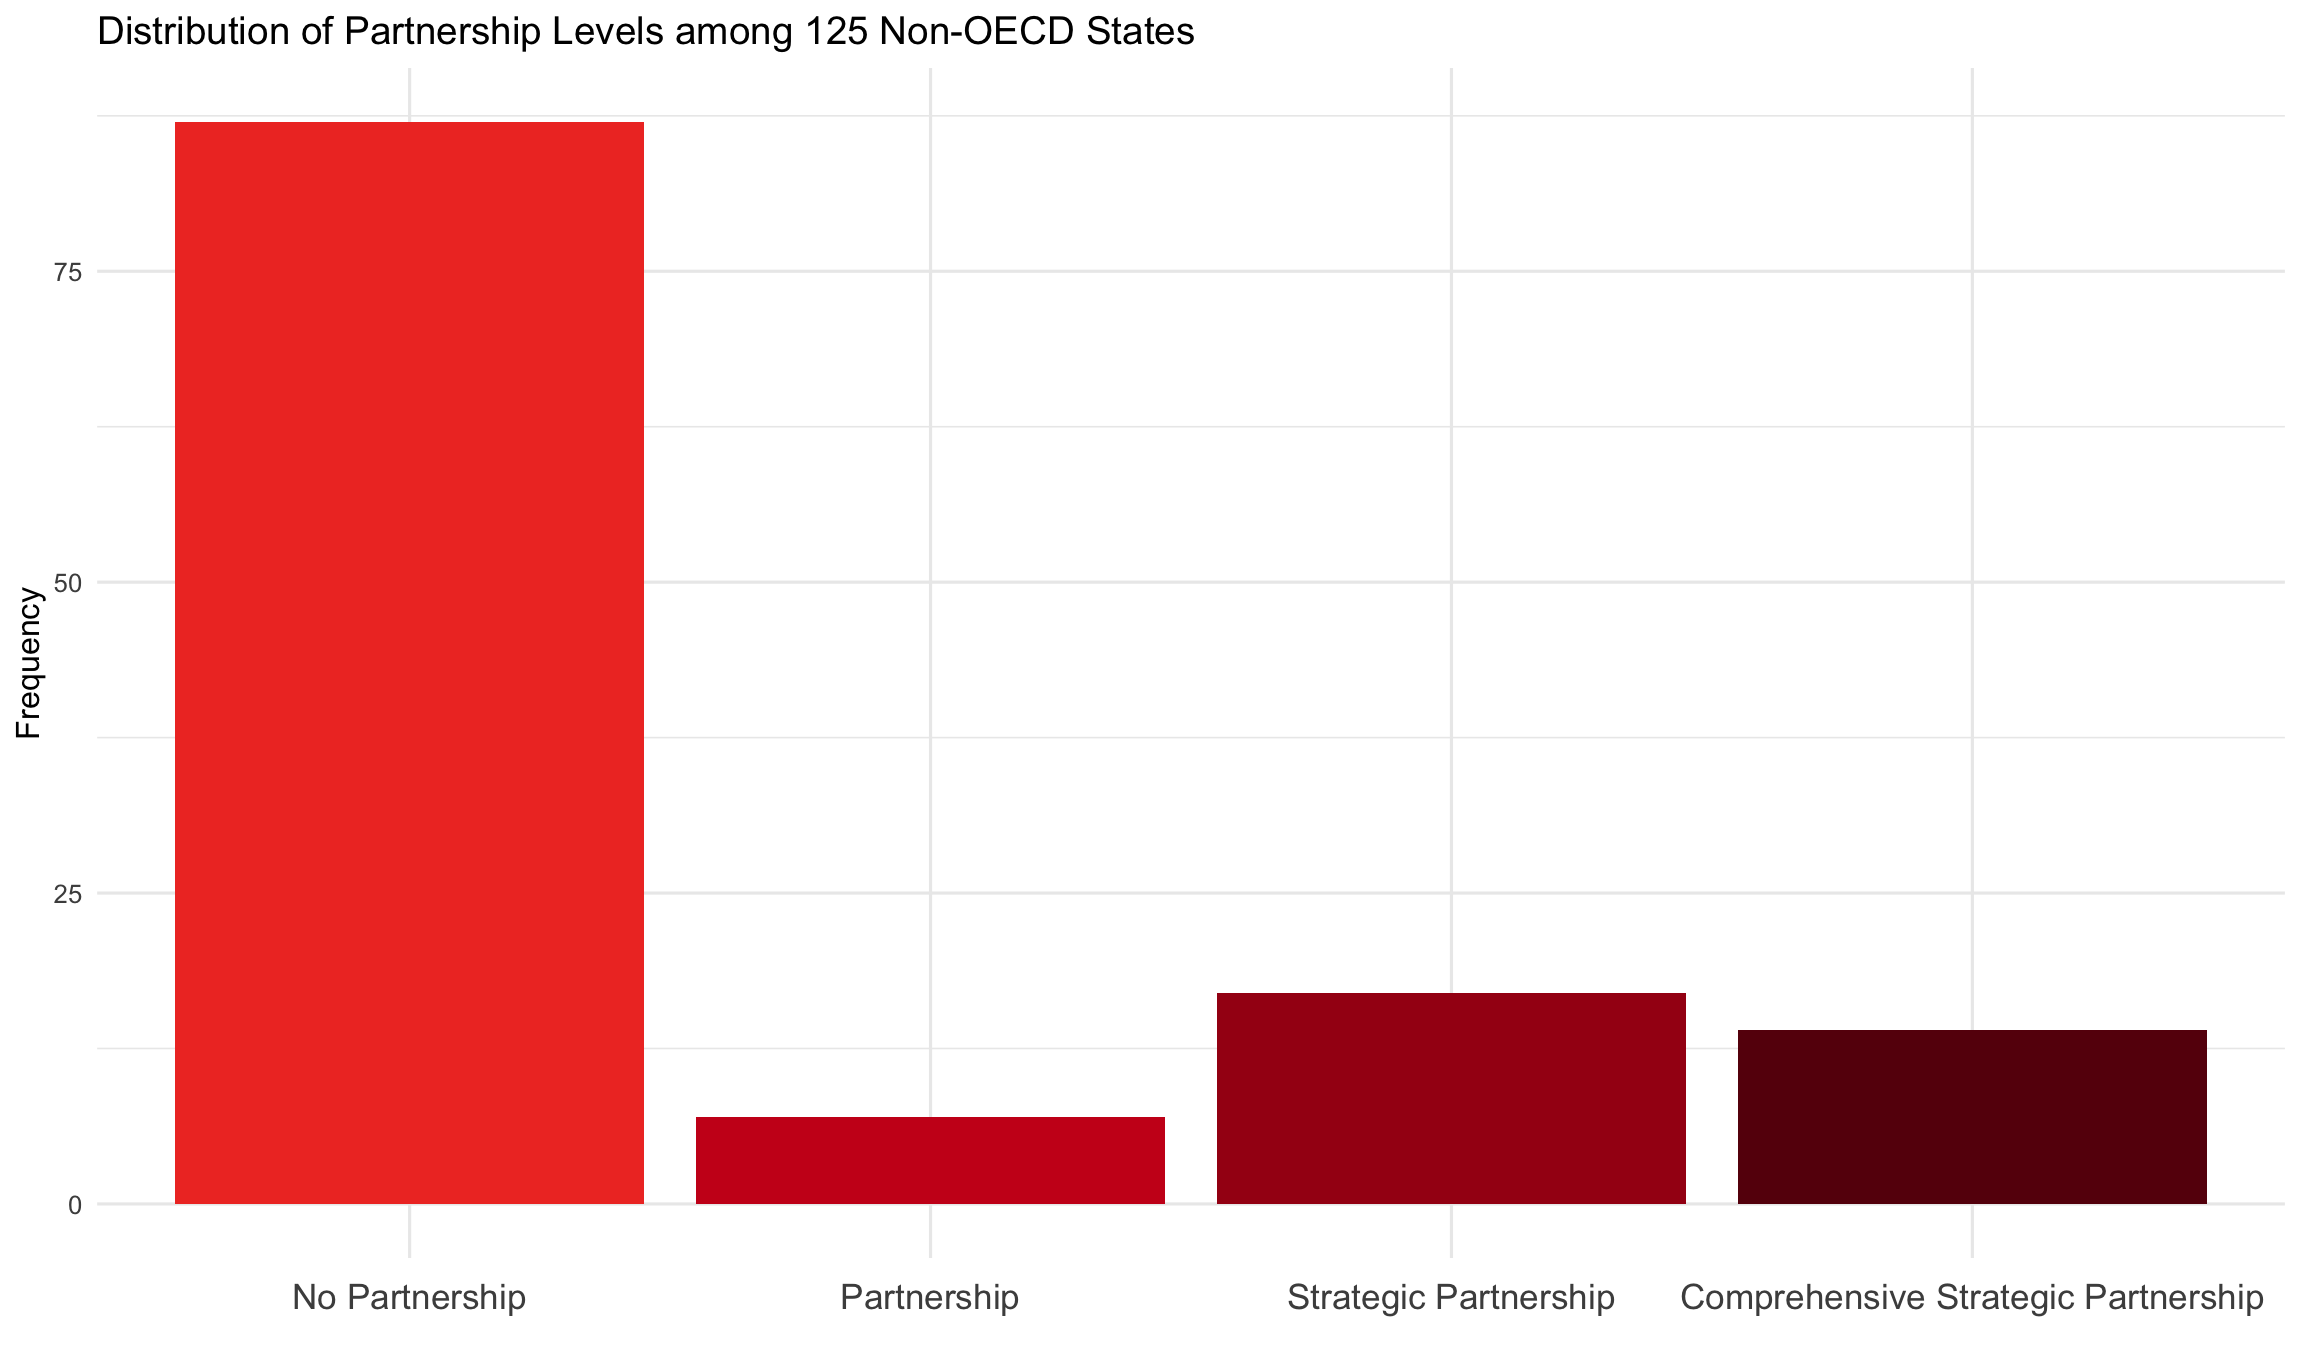
\includegraphics[width=1\linewidth]{plot125.png}
\end{figure}

\lstinputlisting[language=R, firstline=133, lastline=144]{Twist_Lee_MS.R}  

\begin{table}[H] \centering 
  \caption{Original Model 1 (exponentiated)} 
  \label{} 
\begin{tabular}{@{\extracolsep{5pt}}lc} 
\\[-1.8ex]\hline 
\hline \\[-1.8ex] 
 & \multicolumn{1}{c}{\textit{Dependent variable:}} \\ 
\cline{2-2} 
\\[-1.8ex] & Partnership \\ 
\hline \\[-1.8ex] 
 Oil production & 1.139$^{**}$ \\ 
  & (0.058) \\ 
  & \\ 
 GDP per capita & 0.715 \\ 
  & (0.270) \\ 
  & \\ 
 GDP growth & 0.968 \\ 
  & (0.089) \\ 
  & \\ 
 FDI inflows & 1.299$^{***}$ \\ 
  & (0.081) \\ 
  & \\ 
 Trade importance & 3.678 \\ 
  & (0.826) \\ 
  & \\ 
 Level of democracy & 0.993 \\ 
  & (0.051) \\ 
  & \\ 
 Domestic conflict & 1.223 \\ 
  & (0.138) \\ 
  & \\ 
 US ally & 0.398 \\ 
  & (0.777) \\ 
  & \\ 
 Constant & 0.012$^{**}$ \\ 
  & (2.226) \\ 
  & \\ 
\hline \\[-1.8ex] 
Observations & 125 \\ 
Log Likelihood & $-$55.546 \\ 
Residual Deviance & 111.09 \\
AIC & 129.091 \\ 
BIC & 154.5459 \\ 
\hline 
\hline \\[-1.8ex] 
\textit{Note:}  & \multicolumn{1}{r}{$^{*}$p$<$0.1; $^{**}$p$<$0.05; $^{***}$p$<$0.01} \\ 
\end{tabular} 
\end{table} 

\newpage
\lstinputlisting[language=R, firstline=146, lastline=153]{Twist_Lee_MS.R} 

\begin{figure}[H]
    \centering
    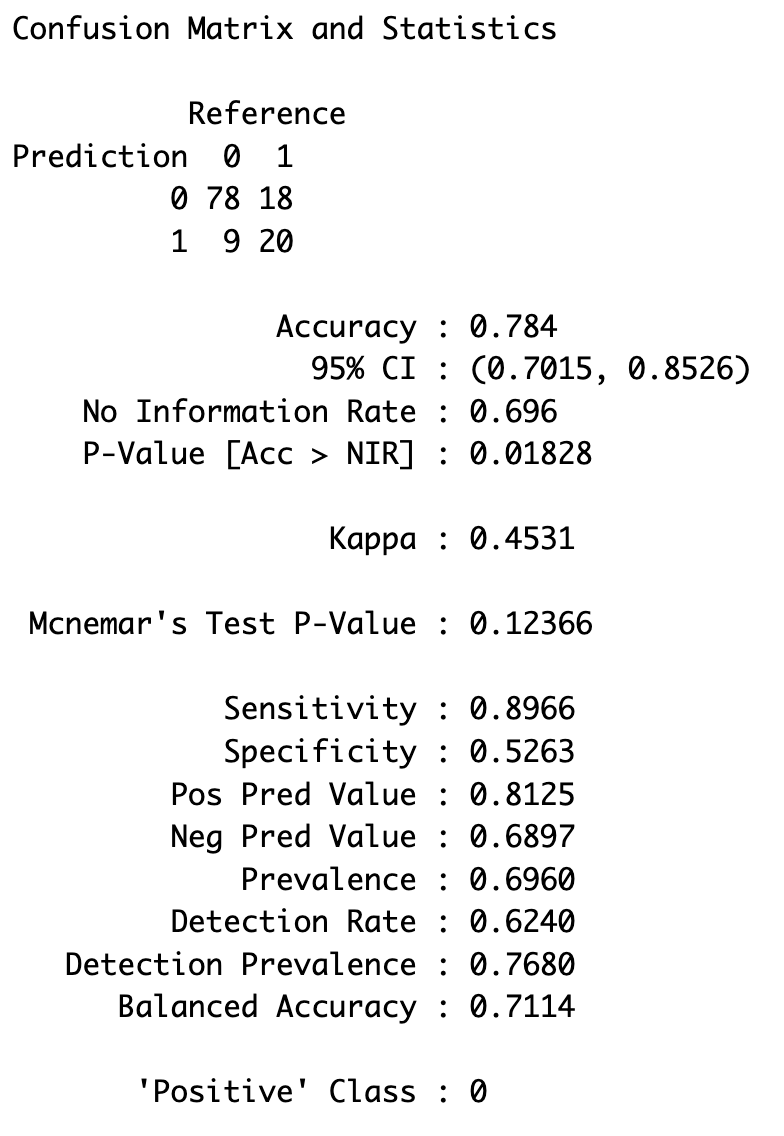
\includegraphics[width=0.5\linewidth]{cm_model1.png}
\end{figure}

\lstinputlisting[language=R, firstline=155, lastline=167]{Twist_Lee_MS.R} 

\begin{figure}[H]
    \centering
    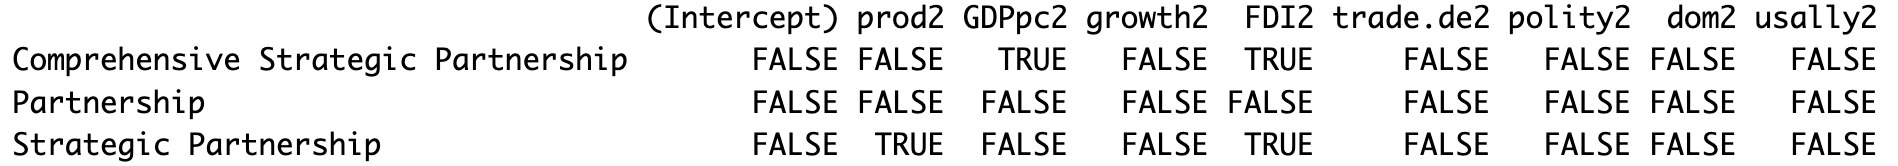
\includegraphics[width=1\linewidth]{pvalues_unord.png}
\end{figure}

\lstinputlisting[language=R, firstline=169, lastline=174]{Twist_Lee_MS.R} 

\begin{table}[H] 
\centering 
\caption{Unordered Model (exponentiated)} 
\label{} 
\begin{tabular}{@{\extracolsep{5pt}}lccc} 
\\[-1.8ex]\hline 
\hline \\[-1.8ex] 
 & \multicolumn{3}{c}{\textit{Dependent variable:}} \\ 
\cline{2-4} 
\\[-1.8ex] & Comprehensive Strategic Partnership & Partnership & Strategic Partnership \\ 
\\[-1.8ex] & (1) & (2) & (3)\\ 
\hline \\[-1.8ex] 
 Oil production & 1.221** & 1.013 & 1.197** \\ 
  & (0.104) & (0.105) & (0.083) \\ 
  & & & \\ 
 GDP per capita & 0.347** & 1.004 & 0.756 \\ 
  & (0.520) & (0.490) & (0.363) \\ 
  & & & \\ 
 GDP growth & 1.003 & 0.864 & 0.980 \\ 
  & (0.157) & (0.227) & (0.103) \\ 
  & & & \\ 
 FDI inflows & 1.885** & 1.133 & 1.266** \\ 
  & (0.284) & (0.148) & (0.097) \\ 
  & & & \\ 
 Trade importance & 10.218** & 0.153 & 2.253 \\ 
  & (1.189) & (4.021) & (1.083) \\ 
  & & & \\ 
 Level of democracy & 0.944 & 1.095 & 0.973 \\ 
  & (0.087) & (0.106) & (0.067) \\ 
  & & & \\ 
 Domestic conflict & 0.957 & 1.308 & 1.337 \\ 
  & (0.239) & (0.236) & (0.177) \\ 
  & & & \\ 
 US ally & 1.536 & 0.230 & 0.288 \\ 
  & (1.268) & (1.281) & (1.047) \\ 
  & & & \\ 
 Constant & 0.000 & 0.008 & 0.003** \\ 
  & (5.576) & (3.694) & (2.928) \\ 
  & & & \\ 
\hline \\[-1.8ex] 
Observations & 125 \\
Log Likelihood & -83.263\\
Residual Deviance & 166.526\\
AIC & 220.526  \\ 
BIC & 296.89 \\
\hline 
\hline \\[-1.8ex] 
\textit{Note:}  & \multicolumn{3}{r}{$^{*}$p$<$0.1; $^{**}$p$<$0.05; $^{***}$p$<$0.01} \\ 
\end{tabular} 
\end{table}

\lstinputlisting[language=R, firstline=176, lastline=181]{Twist_Lee_MS.R} 

\begin{figure}[H]
    \centering
    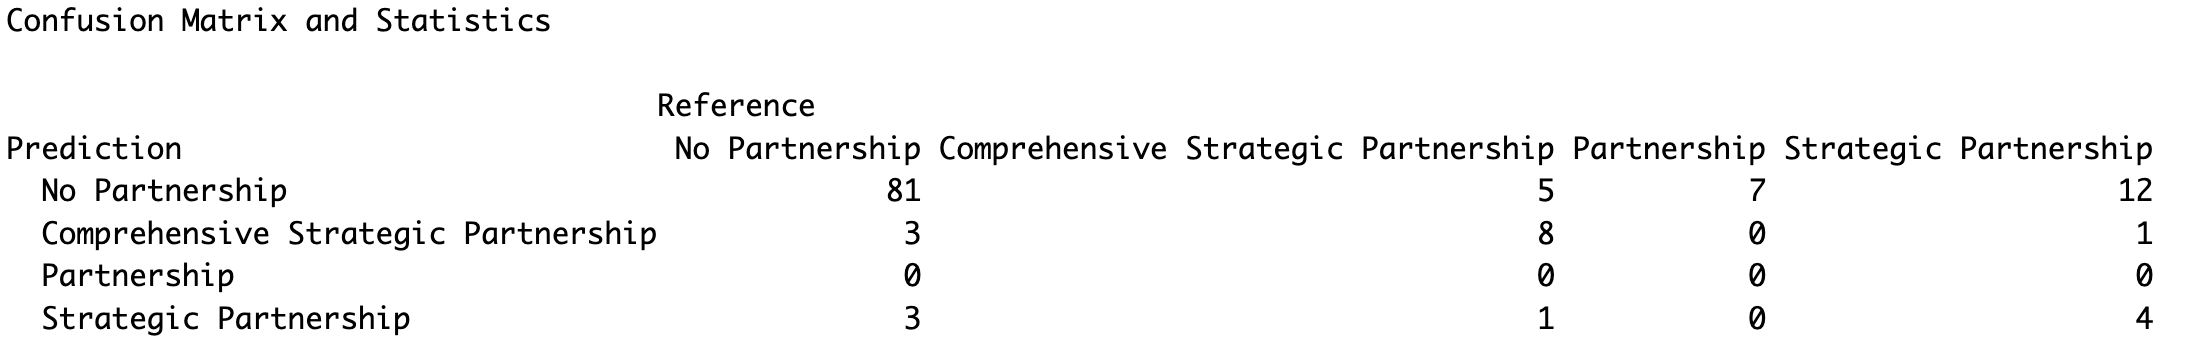
\includegraphics[width=1\linewidth]{cm_unordmodel1.png}
\end{figure}

\begin{figure}[H]
    \centering
    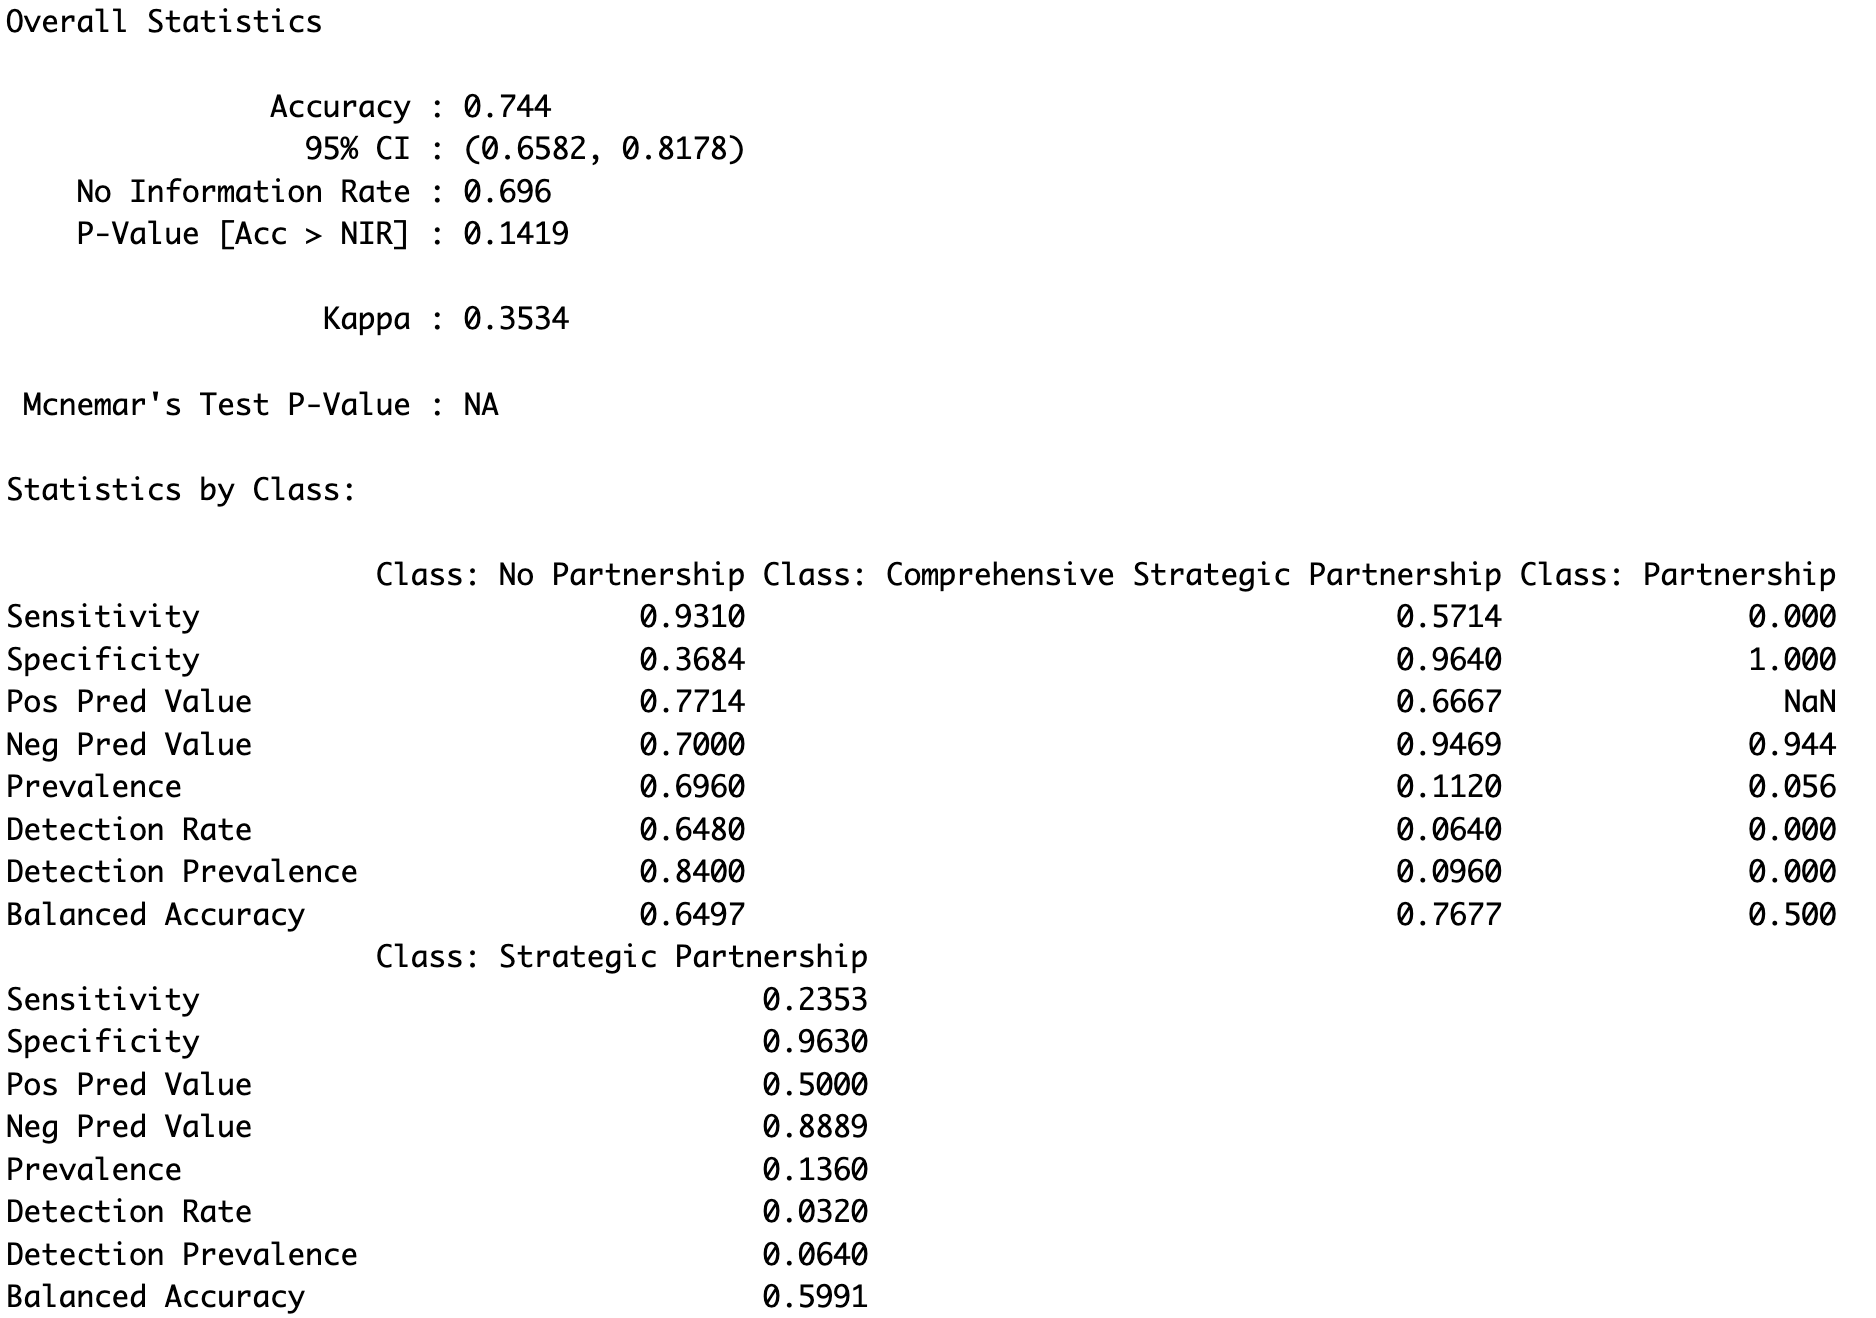
\includegraphics[width=1\linewidth]{cm_unordmodel2.png}
\end{figure}

\lstinputlisting[language=R, firstline=183, lastline=201]{Twist_Lee_MS.R} 

\begin{figure}[H]
    \centering
    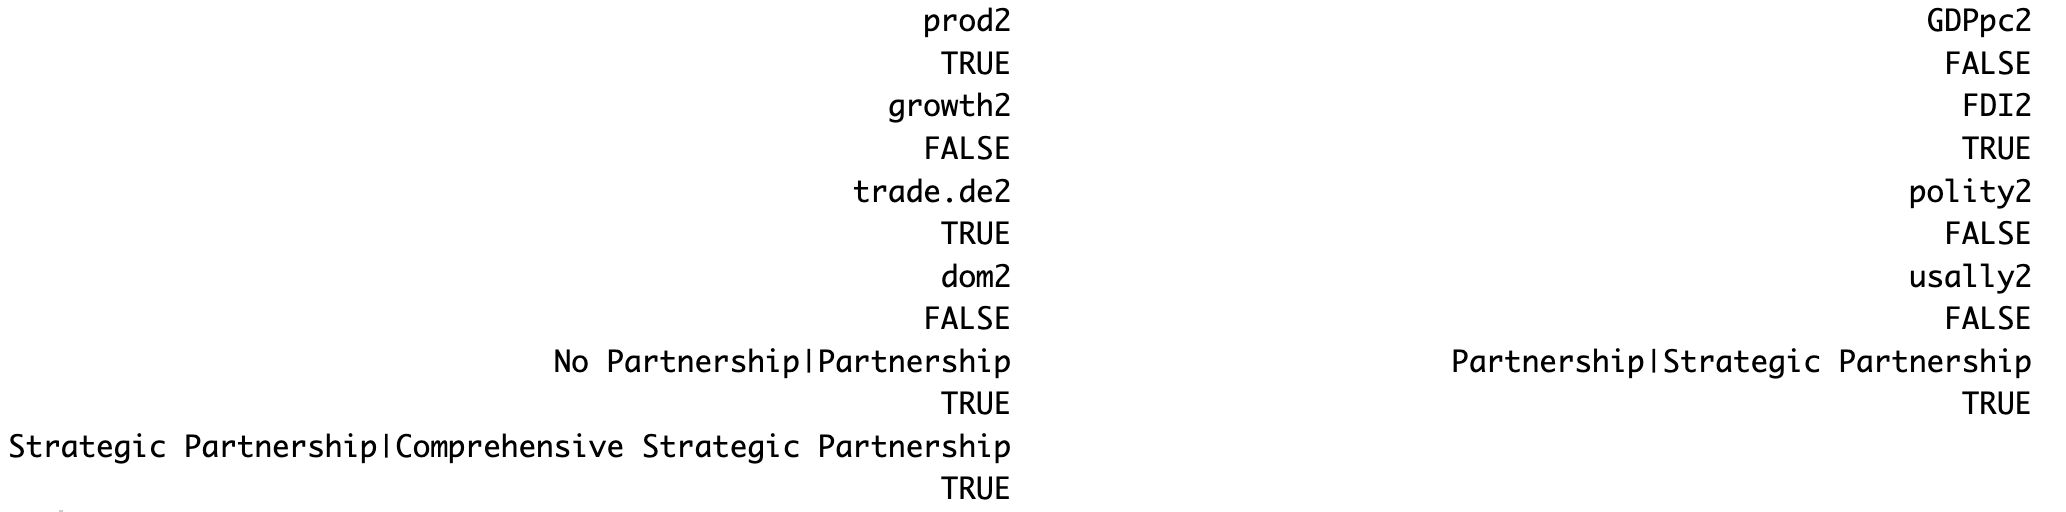
\includegraphics[width=1\linewidth]{pvalues_ord.png}
\end{figure}

\lstinputlisting[language=R, firstline=203, lastline=208]{Twist_Lee_MS.R} 

\begin{table}[H]
\centering 
\caption{Ordered Model (exponentiated)} 
\label{} 
\begin{tabular}{@{\extracolsep{5pt}}lc} 
\\[-1.8ex]\hline 
\hline \\[-1.8ex] 
 & \multicolumn{1}{c}{\textit{Dependent variable:}} \\ 
\cline{2-2} 
\\[-1.8ex] & Partnership Level \\ 
\hline \\[-1.8ex] 
 Oil production & 1.124$^{**}$ \\ 
  & (0.057) \\ 
  & \\ 
 GDP per capita & 0.694 \\ 
  & (0.256) \\ 
  & \\ 
 GDP growth & 0.958 \\ 
  & (0.086) \\ 
  & \\ 
 FDI inflows & 1.324$^{***}$ \\ 
  & (0.078) \\ 
  & \\ 
 Trade importance & 6.095$^{**}$ \\ 
  & (0.745) \\ 
  & \\ 
 Level of democracy & 0.953 \\ 
  & (0.050) \\ 
  & \\ 
 Domestic conflict & 1.155 \\ 
  & (0.131) \\ 
  & \\ 
 US ally & 0.841 \\ 
  & (0.678) \\ 
  & \\ 
\hline \\[-1.8ex] 
\textit{Intercepts} \\
\hline
\hline
No Partnership|Partnership & 77.138**  \\
Partnership|Strategic Partnership & 118.238**  \\
Strategic Partnership|Comprehensive Strategic Partnership & 513.783** \\
\hline
Observations & 125 \\ 
Log Likelihood & $-$90.19376 \\ 
Residual Deviance & 180.3875 \\
AIC & 202.3875 \\ 
BIC & 233.499 \\ 
\hline 
\hline \\[-1.8ex] 
\textit{Note:}  & \multicolumn{1}{r}{$^{*}$p$<$0.1; $^{**}$p$<$0.05; $^{***}$p$<$0.01} \\ 
\end{tabular}
\end{table}

\newpage
\lstinputlisting[language=R, firstline=210, lastline=215]{Twist_Lee_MS.R} 

\begin{figure}[H]
    \centering
    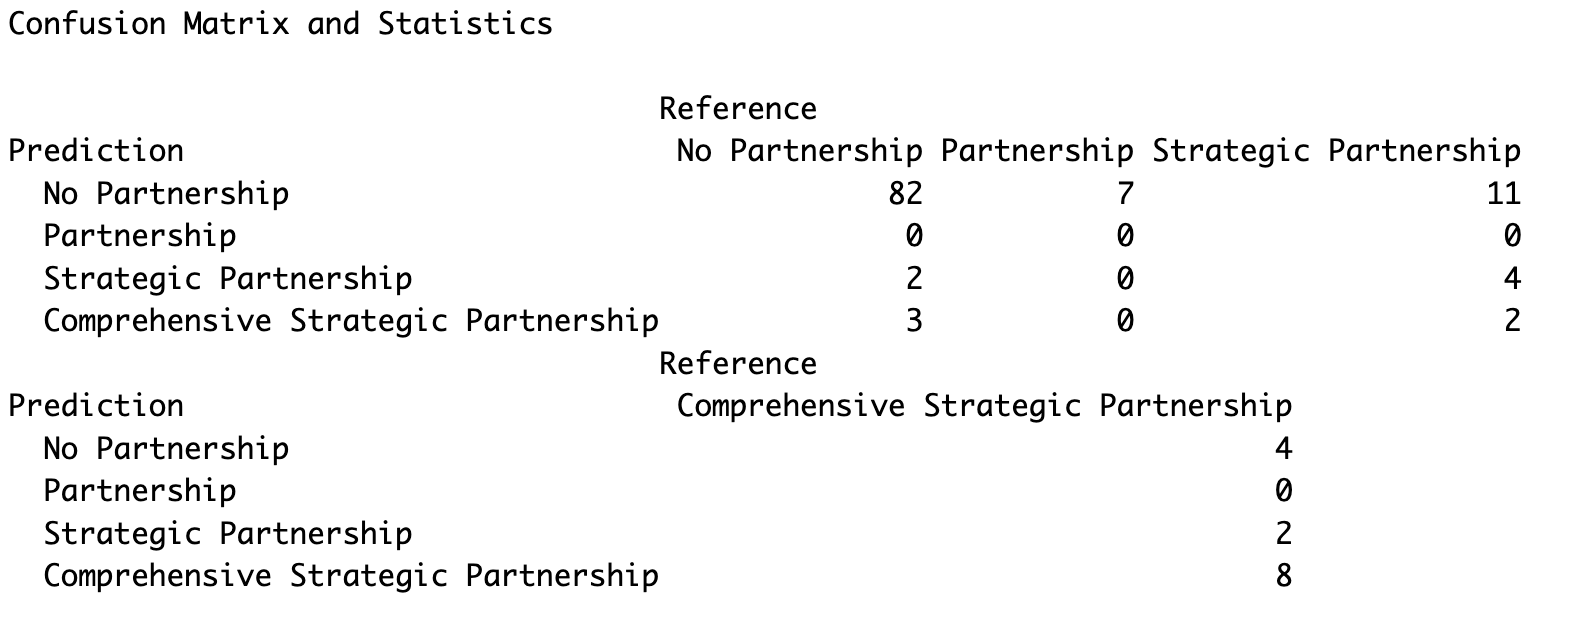
\includegraphics[width=1\linewidth]{cm_ordmodel1.png}
\end{figure}

\begin{figure}[H]
    \centering
    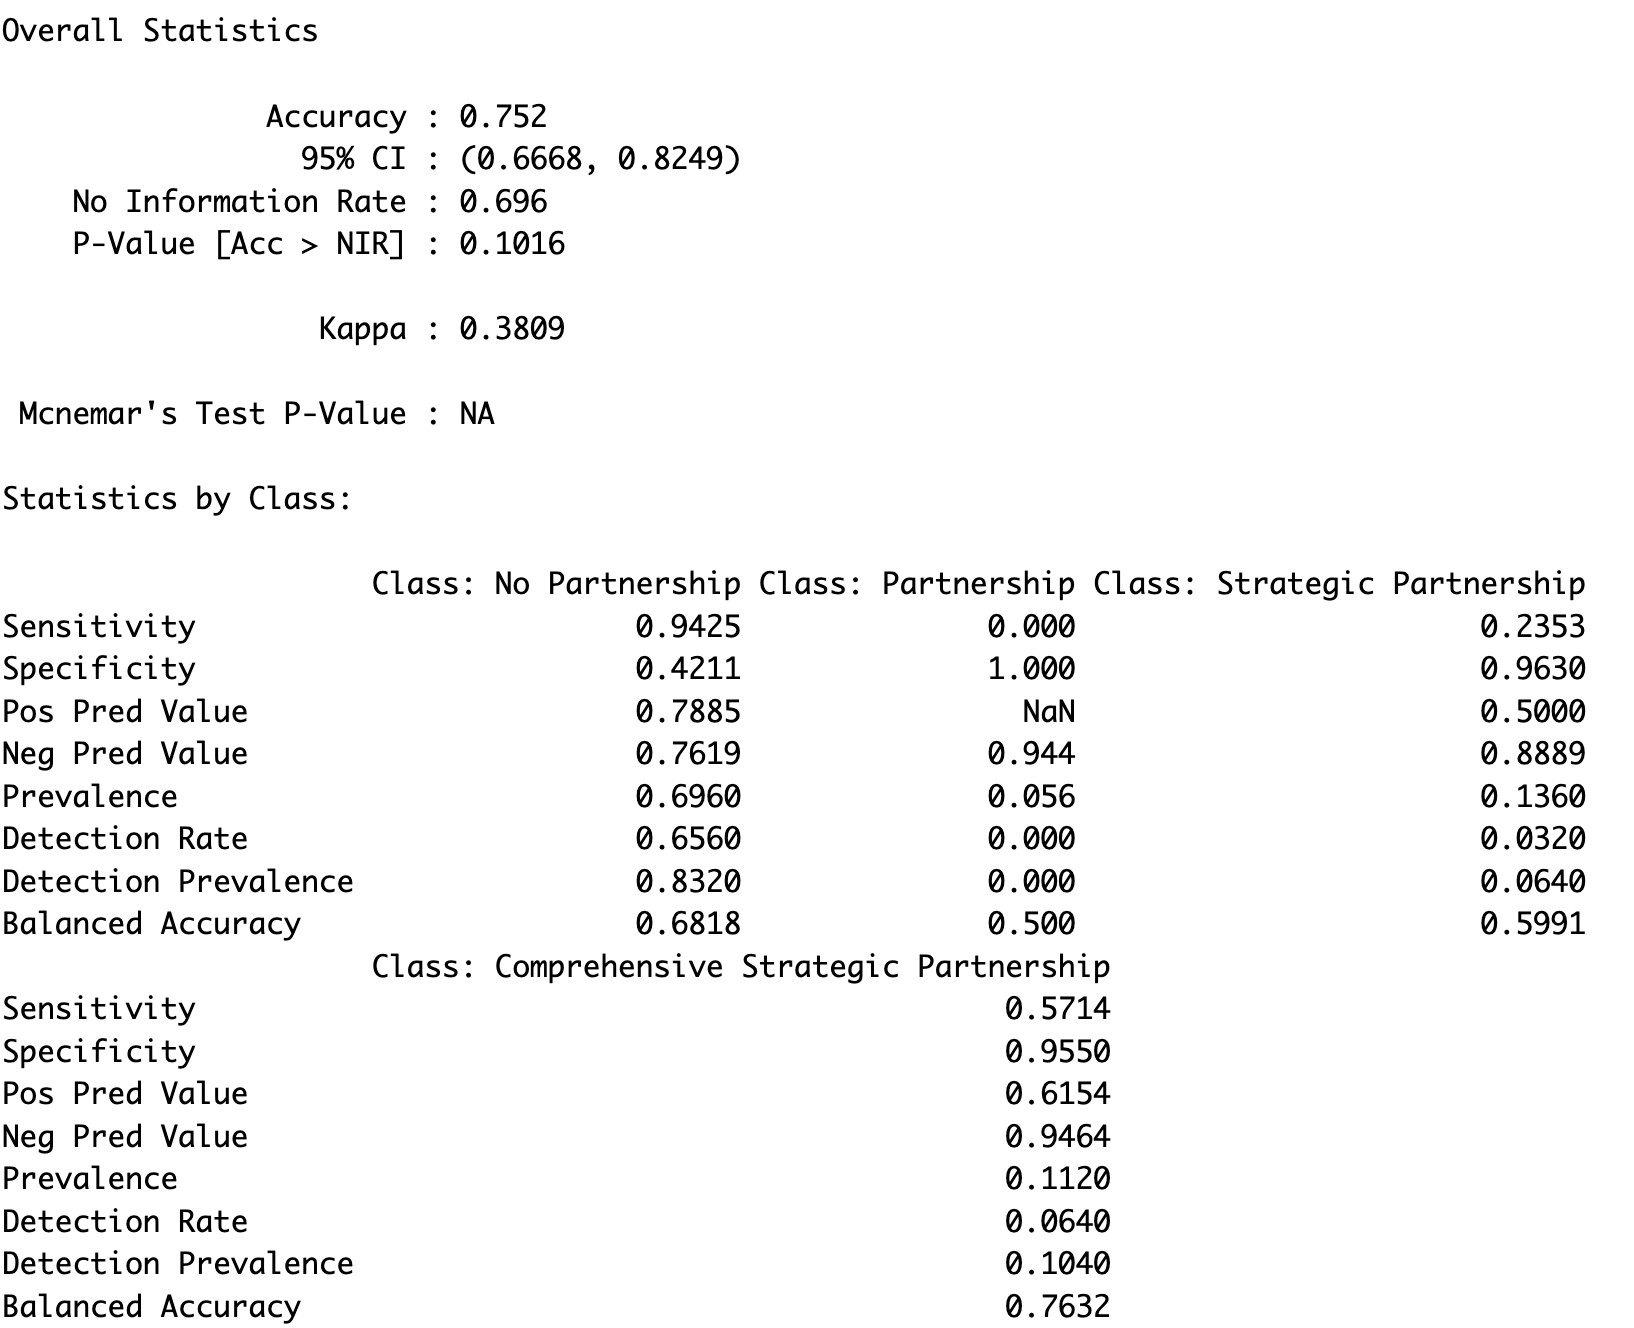
\includegraphics[width=1\linewidth]{cm_ordmodel2.png}
\end{figure}

\lstinputlisting[language=R, firstline=217, lastline=221]{Twist_Lee_MS.R} 
\begin{verbatim}
[1] 166.5255
[1] 180.3875
[1] 111.0911
\end{verbatim}

\lstinputlisting[language=R, firstline=223, lastline=226]{Twist_Lee_MS.R} 
\begin{verbatim}
[1] 129.0911
[1] 220.5255
[1] 202.3875
\end{verbatim}

\lstinputlisting[language=R, firstline=228, lastline=231]{Twist_Lee_MS.R} 
\begin{verbatim}
[1] 154.5459
[1] 296.89
[1] 233.499
\end{verbatim}

\lstinputlisting[language=R, firstline=233, lastline=234]{Twist_Lee_MS.R} 

\begin{figure}[H]
    \centering
    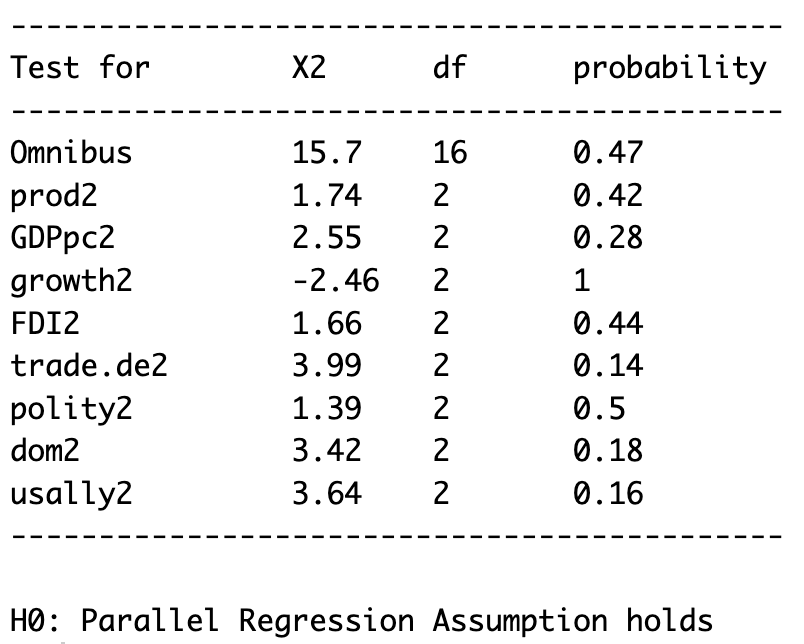
\includegraphics[width=0.5\linewidth]{brant.png}
\end{figure}

\newpage
\section{References}

\noindent Lee, C. (2019). China’s Energy Diplomacy: Does Chinese Foreign Policy Favor Oil-Producing Countries? \textit{Foreign Policy Analysis}, \textbf{15}(4), 570–588. \url{https://doi.org/10.1093/fpa/orz011} \\

\vspace{0.25cm}

\noindent Lee, C. (2023). "Replication data for 'China's Energy Diplomacy: Does Chinese Foreign Policy Favor Oil Producing Countries?'" [Data set]. Harvard Dataverse. \url{https://doi.org/10.7910/DVN/7E3O5P}, V1, UNF:6:x+exuF4WVfknqWQhUWz4MQ== [fileUNF].

\end{document}
